% Results

\chapter{Results} % Main chapter title

\label{Results} % For referencing the chapter elsewhere, use \ref{Chapter1} 

\lhead{Chapter 6. \emph{Tests and results}} % This is for the header on each page - perhaps a shortened title

In this chapter, we will describe and discuss our experimental results in order to validate our system and bring it to face to previous studies.
 
%----------------------------------------------------------------------------------------
%	METHODOLOGY
%----------------------------------------------------------------------------------------

\section{Experimental setup}

We propose to evaluate different aspects and characteristics of our system considering an indoor communication situation avoiding sunlight perturbations.

In addition, we consider different cases: with or without ambient light interferences, Manchester or 4B6B coding, changing the clock rate and the emitter distance from the receiver. 

\section{Protocol}

The receiver was placed in a fix position, while the LED light source keep mobile. In that way, the distance between the emitter and the receiver can  be changed. To keep the measure consistent, we place a luxmeter, just near the receiver to approximate the effective illumination.

During the probes, both emitter and receiver micro-controller were connected with their debugging interface to a laptop, on a side to change the LED driver parameters, and on other side to visualize and record received data at different place of our system. 

In addition, we used on oscilloscope to check the circuit output and control the signal generated by the emitter micro-controller.

The emitter light was alimented with a 28 Volts power supply and the LED Driver has been programmed to send periodically a 16-bits counter value, with the pattern defined in \ref{frame}.

About the distance/illumination, probes have been realized in a range of 75 to 300 centimeters to match an indoor possible usage. On other side, the clock frequency has been limited to 560kHz, considering the ADC sampling rate - 1,1 MSPS - and the Nyquist-Shannon sampling theorem : 
\begin{equation}
f_{Nyquist}  = \frac{f_{sampling}}{2}
\label{eq:nyquist}
\end{equation}

\begin{figure}[htbp]
  \centering
    \makebox[\textwidth][c]{
      \scalebox{0.4}{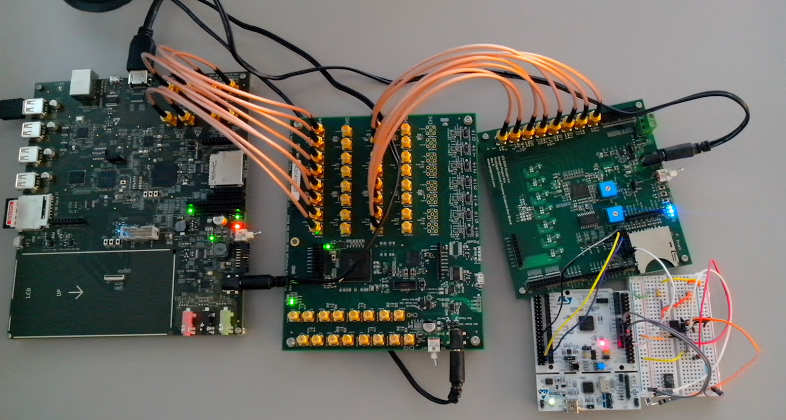
\includegraphics{Pictures/receiver_setup.jpg}
    }}
    \rule{35em}{0.5pt}
  \caption[The ARA MDK and its VLC receiver module]{The ARA MDK and its VLC receiver module}
  \label{fig:receiver}
\end{figure}

\begin{figure}[htbp]
	\centering
	\makebox[\textwidth][c]{
		\scalebox{0.3}{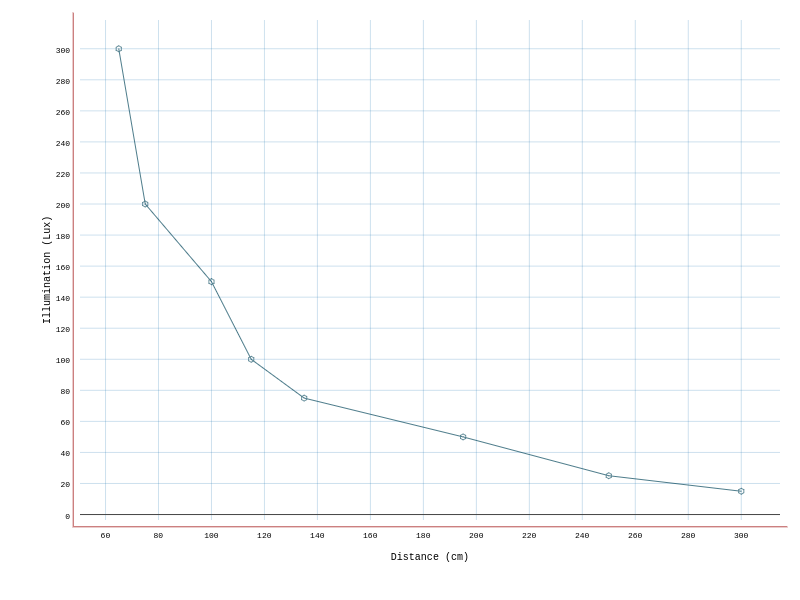
\includegraphics{Pictures/led.png}
	}}
		\rule{35em}{0.5pt}
		\caption{Receiver illumination over the distance}
		\label{fig:led}
	\end{figure}

\section{Circuit Evaluation}

The received signal was measured at different steps of the analogical processing, using the 2 oscilloscope voices at different points of our circuit. The high-pass filter and adjustments made on the receiver front-end circuit are satisfactory, and improve the signal quality before sampling.

\begin{figure}[htbp]
	\centering
	\makebox[\textwidth][c]{
		\scalebox{0.6}{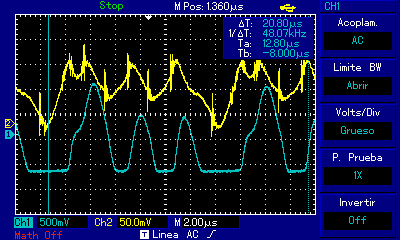
\includegraphics{Pictures/circuit-compare.png}
	}}
		\rule{35em}{0.5pt}
		\caption[In yellow the signal just after the TIA. In blue, the signal after analogical filtering - 2,5 meter distance]{In yellow the signal just after the TIA. In blue, the signal after analogical filtering - 2,5 meter distance}
		\label{fig:circuit-compare}
	\end{figure}
	
section{Digitalization and demodulation}

In order evaluate our demodulation and digital processing algorithms, we plot the sampled signal and the bits obtained after computation. We can see in the figure \ref{fig:numeric} that it is correct and we can get rid of signal attenuation due to circuit latency.
\begin{figure}[htbp]
	\centering
	\makebox[\textwidth][c]{
		\scalebox{0.4}{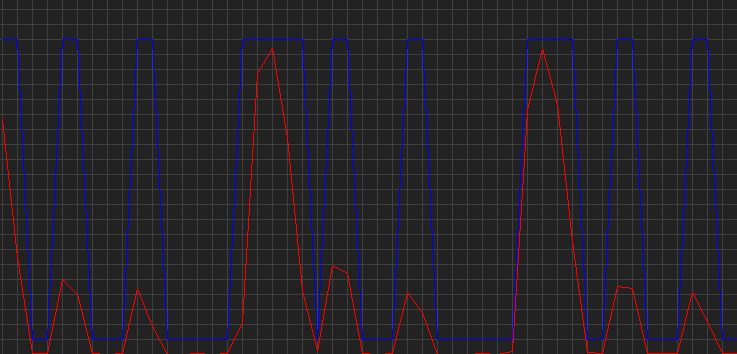
\includegraphics{Pictures/numerized.png}
	}}
		\rule{35em}{0.5pt}
		\caption{In red the signal sampled. In blue, the bits computed after digital processing and demodulation}
		\label{fig:numeric}
	\end{figure}

\section{Bit Error Rate}

In digital transmission, the number of bit errors is the number of received bits of a data stream over a communication channel that have been altered due to noise, interference, distortion or bit synchronization errors.

As we know exactly the sequence of bit that have been emitted and the decoded sequence, we were able to compute it, for different illumination level and clock-rate, using Manchester or 4B6B coding.

\subsection{4B6B}

\begin{table}[htbp]
\begin{center}
\begin{tabular}{|c|c|c|}
  \hline
  clock rate (kHz) & bitrate (kbps) & BER \\
  \hline
  100 & 67 & $<$ 10$^-4$ \\
  160 & 107 & $<$ 10$^-4$ \\
  240 & 160 & 3.10$^-4$ \\
  380 & 253 & 6.10$^-4$ \\
  560 & 373 & 2.10$^-2$ \\
  \hline
\end{tabular}
\end{center}
\caption{Bit Error Rate for different clock rate at 2,5 meters, using 4B6B coding}
\label{tab:ber}
\end{table}

Considering table \ref{tab:ber} 2,5 meters distance and 10$^-3$ as admissible BER, we can assume that using a 380kHz clock rate can be used for a correct transmission using 4B6B.

In that case, with 4B6B coding, we obtain a raw throughput of 253 kbps.

\subsection{Manchester}
Using Manchester coding, we obtained a surge of the bit error rate when the illumination is lower than 100 Lux. Analyzing the signal at the ADC input, we put in evidence that this is due to wave attenuation : isolated bit, just after long sequences are not detected, as visible in the figure \ref{fig:manchester-problem}.

\begin{table}[htbp]
\begin{center}
\begin{tabular}{|c|c|c|}
  \hline
  clock rate (kHz) & bitrate (kbps) & BER \\
  \hline
  100 & 50 & $<$ 10$^-4$ \\
  160 & 80 & $<$ 10$^-4$ \\
  240 & 120 & 8.10$^-4$ \\
  380 & 190 & 4.10$^-2$ \\
  560 & 280 & $>$ 10$^-1$ \\
  \hline
\end{tabular}
\end{center}
\caption{Bit Error Rate for different clock rate at 2,5 meters, using Manchester coding}
\label{tab:ber-manchester}
\end{table}

\begin{figure}[htbp]
	\centering
	\makebox[\textwidth][c]{
		\scalebox{0.6}{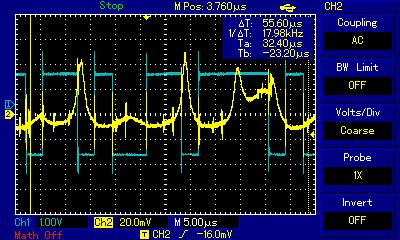
\includegraphics{Pictures/manchester-prob.jpg}
	}}
		\rule{35em}{0.5pt}
		\caption
        {In blue, the signal generated by the LED driver. In yellow, the signal after our circuit - 2,5 meter distance - 360kHz}
		\label{fig:manchester-problem}
	\end{figure}
    
 
%----------------------------------------------------------------------------------------
%	RESULTS AND INTERPRETATION-----------------------

%-----------------------------------------------------------------
\section{Discussion}

Regarding previous results, we were able to validate our proposal. We can achieve a reliable transmission between a commercial LED and the modular smartphone at a suitable distance for indoor usage.

Comparing our  module for ARA platform with previous system, such \citep{phycomp}, or other proposal using the smartphone camera and rolling shutter effect  \citep{rolling}, we obtained and recorded an higher bitrate, up to 253 kbps.
\citep{phycomp}